% This file was created with tikzplotlib v0.10.1.
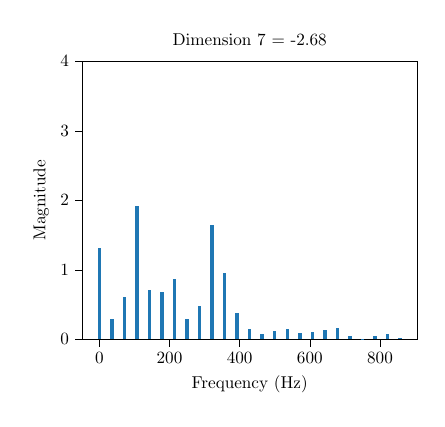
\begin{tikzpicture}[scale=0.62]

\definecolor{darkgray176}{RGB}{176,176,176}
\definecolor{steelblue31119180}{RGB}{31,119,180}

\begin{axis}[
tick align=outside,
tick pos=left,
x grid style={darkgray176},
xlabel={Frequency (Hz)},
xmin=-48.3571428571429, xmax=905.5,
xtick style={color=black},
y grid style={darkgray176},
ylabel={Magnitude},
ymin=0, ymax=4,
title={Dimension 7 = -2.68},
ytick style={color=black}
]
\draw[draw=none,fill=steelblue31119180] (axis cs:-5,0) rectangle (axis cs:5,1.31270937714726);
\draw[draw=none,fill=steelblue31119180] (axis cs:30.7142857142857,0) rectangle (axis cs:40.7142857142857,0.288125975872221);
\draw[draw=none,fill=steelblue31119180] (axis cs:66.4285714285714,0) rectangle (axis cs:76.4285714285714,0.616790952368152);
\draw[draw=none,fill=steelblue31119180] (axis cs:102.142857142857,0) rectangle (axis cs:112.142857142857,1.92312523138079);
\draw[draw=none,fill=steelblue31119180] (axis cs:137.857142857143,0) rectangle (axis cs:147.857142857143,0.707237007629874);
\draw[draw=none,fill=steelblue31119180] (axis cs:173.571428571429,0) rectangle (axis cs:183.571428571429,0.677698119881814);
\draw[draw=none,fill=steelblue31119180] (axis cs:209.285714285714,0) rectangle (axis cs:219.285714285714,0.862386040544995);
\draw[draw=none,fill=steelblue31119180] (axis cs:245,0) rectangle (axis cs:255,0.298711415685218);
\draw[draw=none,fill=steelblue31119180] (axis cs:280.714285714286,0) rectangle (axis cs:290.714285714286,0.483968708976862);
\draw[draw=none,fill=steelblue31119180] (axis cs:316.428571428571,0) rectangle (axis cs:326.428571428571,1.65269155101225);
\draw[draw=none,fill=steelblue31119180] (axis cs:352.142857142857,0) rectangle (axis cs:362.142857142857,0.951122100407993);
\draw[draw=none,fill=steelblue31119180] (axis cs:387.857142857143,0) rectangle (axis cs:397.857142857143,0.377021033569998);
\draw[draw=none,fill=steelblue31119180] (axis cs:423.571428571429,0) rectangle (axis cs:433.571428571429,0.156449857538637);
\draw[draw=none,fill=steelblue31119180] (axis cs:459.285714285714,0) rectangle (axis cs:469.285714285714,0.0846393619854383);
\draw[draw=none,fill=steelblue31119180] (axis cs:495,0) rectangle (axis cs:505,0.118818944486802);
\draw[draw=none,fill=steelblue31119180] (axis cs:530.714285714286,0) rectangle (axis cs:540.714285714286,0.143214948815801);
\draw[draw=none,fill=steelblue31119180] (axis cs:566.428571428571,0) rectangle (axis cs:576.428571428571,0.0949080699867579);
\draw[draw=none,fill=steelblue31119180] (axis cs:602.142857142857,0) rectangle (axis cs:612.142857142857,0.10757439472035);
\draw[draw=none,fill=steelblue31119180] (axis cs:637.857142857143,0) rectangle (axis cs:647.857142857143,0.131395993038413);
\draw[draw=none,fill=steelblue31119180] (axis cs:673.571428571429,0) rectangle (axis cs:683.571428571429,0.160127533802761);
\draw[draw=none,fill=steelblue31119180] (axis cs:709.285714285714,0) rectangle (axis cs:719.285714285714,0.0535699464522896);
\draw[draw=none,fill=steelblue31119180] (axis cs:745,0) rectangle (axis cs:755,0.00967304476823895);
\draw[draw=none,fill=steelblue31119180] (axis cs:780.714285714286,0) rectangle (axis cs:790.714285714286,0.0422317493349039);
\draw[draw=none,fill=steelblue31119180] (axis cs:816.428571428571,0) rectangle (axis cs:826.428571428571,0.0743497564419976);
\draw[draw=none,fill=steelblue31119180] (axis cs:852.142857142857,0) rectangle (axis cs:862.142857142857,0.0273048386393424);
\end{axis}

\end{tikzpicture}
